\documentclass[a4paper,11pt]{article}

% Kodovani (cestiny) v dokumentu: utf-8
%\usepackage[cp1250]{inputenc}	% Omezena stredoevropska kodova stranka, pouze MSW.
\usepackage[utf8]{inputenc}	% Doporucujeme pouzivat UTF-8 (unicode).

\usepackage[margin=2cm]{geometry}
\newtoks\jmenopraktika \newtoks\jmeno \newtoks\datum
\newtoks\obor \newtoks\skupina \newtoks\rocnik \newtoks\semestr
\newtoks\cisloulohy \newtoks\jmenoulohy
\newtoks\tlak \newtoks\teplota \newtoks\vlhkost

\jmenopraktika={Fyzikální praktikum 1}
\jmeno={Lukáš Lejdar}
\datum={1. října 2024}
\obor={F}
\skupina={Út 16:00}

\cisloulohy={6}
\jmenoulohy={Elektromagnetické kmity v RLC obvodu}

\tlak={101{,}35}
\teplota={21,1}
\vlhkost={47,7}

%%%%%%%%%%% Uzitecne balicky:
\usepackage[czech]{babel}
\addto\captionsczech{\renewcommand{\figurename}{Obrázek}}

\usepackage{graphicx}
\usepackage{amsmath}
\usepackage{xspace}
\usepackage{url}
\usepackage{indentfirst}
\usepackage{wrapfig}
\usepackage{xcolor}
\usepackage{subfig}
\usepackage{subcaption}
\usepackage{enumitem}
\usepackage{tikzsymbols}
\usepackage{mathtools}
\usepackage{newfloat}

\DeclareFloatingEnvironment[fileext=lof]{graph}
\captionsetup[graph]{labelformat=simple, labelsep=colon, name=Graf}

%%%%%% Zamezeni parchantu:
\widowpenalty 10000 \clubpenalty 10000 \displaywidowpenalty 10000
%%%%%% Parametry pro moznost vsazeni vetsiho poctu obrazku na stranku
\setcounter{topnumber}{3}	  % max. pocet floatu nahore (specifikace t)
\setcounter{bottomnumber}{3}	  % max. pocet floatu dole (specifikace b)
\setcounter{totalnumber}{6}	  % max. pocet floatu na strance celkem
\renewcommand\topfraction{0.9}	  % max podil stranky pro floaty nahore
\renewcommand\bottomfraction{0.9} % max podil stranky pro floaty dole
\renewcommand\textfraction{0.1}	  % min podil stranky, ktery musi obsahovat text
\intextsep=8mm \textfloatsep=8mm  %\intextsep pro ulozeni [h] floatu a \textfloatsep pro [b] or [t]

% Tecky za cisly sekci:
\renewcommand{\thesection}{\arabic{section}.}
\renewcommand{\thesubsection}{\thesection\arabic{subsection}.}
% Jednopismenna mezera mezi cislem a nazvem kapitoly:
\makeatletter \def\@seccntformat#1{\csname the#1\endcsname\hspace{1ex}} \makeatother
%
\newcommand{\vsn}[4]{\ensuremath{#1 =} #2(#3)\,#4}
\newcommand{\vrn}[6]{\ensuremath{#1 =} (#2 $\pm$ #3)\,#4 ($p=$ #5\,\%, $\nu=$ #6)}

\newcommand*\circled[1]{\tikz[baseline=(char.base)]{
		\node[shape=circle,draw,inner sep=1pt] (char) {#1};}}

%%%%%%%%%%%%%%%%%%%%%%%%%%%%%%%%%%%%%%%%%%%%%%%%%%%%%%%%%%%%%%%%%%%%%%%%%%%%%%%
% Zacatek dokumentu
%%%%%%%%%%%%%%%%%%%%%%%%%%%%%%%%%%%%%%%%%%%%%%%%%%%%%%%%%%%%%%%%%%%%%%%%%%%%%%%

\begin{document}

\thispagestyle{empty}

{
\begin{center}
\sf 
{\Large Ústav fyziky a technologií plazmatu Přírodovědecké fakulty Masarykovy univerzity} \\
\bigskip
{\huge \bfseries FYZIKÁLNÍ PRAKTIKUM} \\
\bigskip
{\Large \the\jmenopraktika}
\end{center}

\bigskip

\sf
\noindent
\setlength{\arrayrulewidth}{1pt}
\begin{tabular*}{\textwidth}{@{\extracolsep{\fill}} l l}
\large {\bfseries Zpracoval:}  \the\jmeno & \large  {\bfseries Naměřeno:} \the\datum\\[2mm]
\large  {\bfseries Obor:} \the\obor  \hspace{40mm}  {\bfseries Skupina:} \the\skupina %
&\large {\bfseries Testováno:}\\
\\
\hline
\end{tabular*}
}

\bigskip

{
\sf
\noindent \begin{tabular}{p{4cm} p{0.6\textwidth}}
\Large  Úloha č. {\bfseries \the\cisloulohy:} \par
\smallskip
$T=\the\teplota$~$^\circ$C \par
$p=\the\tlak$~kPa \par
$\varphi=\the\vlhkost$~\%
&\Large \bfseries \the\jmenoulohy  \\[2mm]
\end{tabular}
}

\vskip1cm

\section{Úvod}

Cílem je změřit frekvenční charakteristiku RLC obvodu a jeho přechodové jevy. Obvod sestavím ze sériově zapojeného odporu, cívky a kondenzátoru, pro které nejdřív zjistím impedanci a fázový posun.

\section{Postup měření}

\subsection{Impedance a fázový posun}

Pro měření impedance $ \hat{Z} $ použiju obvod z obrázku 1 a), kde na funkčním generátor nastavím harmonický průběh napětí $ U_1 = U_{M1} \cos ( \omega t ) $. Po ustálení pak platí

\begin{equation}
    \hat{Z} = \frac{\hat{U}_Z}{\hat{I}} = R_I \frac{\hat{U}_Z}{\hat{U}_I} = R_I \frac{\| \hat{U}_1 - \hat{U}_2 \| }{U_2} e^{i \varphi_Z}.
\end{equation}

Pokud na osciloskopu nastavím rozdíl měřených napětí $ U_1 $ a $ U_2 $, můžu jejich amplitudu a fázový posun zjistit přímo. Odpor, indukčnost a kapacitu potom pro jednotlivé součástky spočítám jako 

%%

\begin{align*}
    \hat{Z}_R = R_R && \hat{Z}_L = R_L + i \omega L  && \hat{Z}_C = R_C + \frac{1}{i \omega C} .
\end{align*}


\begin{figure}[htpb]
    \centering
    \includegraphics[width=0.44\textwidth]{aparatura_a.png}
    \hfill
    \includegraphics[width=0.44\textwidth]{aparatura_b.png}
    \caption{(a) Aparatura pro měření impedance $ \hat{Z} $ (b) pro měření přechodových jevů.}
\end{figure}

\subsection{Frekvenční charakteristika RLC obvodu}

Bude mě zajímat celková impedance RLC obvodu $ \hat{Z} $, v závislosti na nastavené frekvenci $ f = \frac{\omega}{2 \pi} $ harmonického generátoru napětí. Opět použiju zapojení z obrázku 1 a), kde za součástku dosadím sériově zapojený RLC obvod pro odpor, cívku a kondenzátor. Po ustálení platí opět platí (1), kde
\begin{align}
    Z^2 &= R_{\rm celk}^2 + \left(\omega L - \frac{1}{\omega C}\right)^2 \\
    \varphi_Z &= \arctan\left(\frac{ \omega L - \frac{1}{\omega C} }{R_{\rm celk}}\right).
\end{align}

$ Z $ nabývá minima, když $ \omega = \omega_0 = \frac{1}{\sqrt{LC} } $ s odpovídajícím $ \varphi_0 = 0 $. Použiju stejné součástky jako v 1. části a hodnotu $ \omega_0 $ nejdřív spočítám teoreticky. Nastavím frekvenci $ f_0 = \frac{w_0}{2 \pi} $ a v jejím okolí postupně proměřím závislost vodivosti $ G(\omega) = \frac{1}{Z(\omega)} $ a fázový posun $ \varphi(w) $.

\subsection{Přechodové jevy}

Měřit budu na obvodu z obrázku 2 (b), kde na funkčním generátoru nastavím obdélníkové pulzy pro $ U_{\rm low} $ a $ U_{\rm high} $ s takovou frekvencí, aby se obvod pokaždé stihl ustálit než dojde k další změně napětí. V kroku z low na high tak nastává $ U_C(t_0) = U_{\rm low} $, $ I(t_0) = 0 = \dot{U}_C(t_0) C $  a $ U_f = U_{\rm high} $, čímž jsou počáteční podmínky zadané pro $ U_C(t) $, které se tím stává hledanou závislostí.

Pro kmity sériového RLC obvodu při konstantním budícím napětí $ U(t) = U_{\rm high}= U_f $ pak platí

\begin{align}
    L \ddot{U}_C(t) + R \dot{U}_C(t) + \frac{1}{C} U_C(t) &= \frac{1}{C} U_f.
\end{align}

Kořeny charakteristické rovnice najdu jako $ \lambda_{1,2} = -\alpha \pm \omega_d $, kde  $ \omega_d = \sqrt{\omega_0^2 - \alpha^2} $, $ \alpha = \frac{R}{2L} $ a $ \omega_0 = \frac{1}{\sqrt{LC} } $, přičemž rozlišujeme 3 typy řešení 

\begin{flalign}
   &\text{\textbf{\circled{1}} Podkritické s } \alpha > \omega_0 & U_C(t) &= C_1 \cos(\omega_d t+ \varphi) e ^{- \alpha t} + U_f && R_R \approx R > 2 \omega_0 L\\
   &\text{\textbf{\circled{2}} Nadkritické s } \alpha < \omega_0 & U_C(t) &= C_1 \sinh(i \omega_d t + \varphi) e ^{-\alpha t} + U_f && R_R \approx R < 2 \omega_0 L \\
   &\text{\textbf{\circled{3}} Kritické s } \alpha = \omega_0 & U_C(t) &= (U_i - U_f) (1 + \alpha t)e ^{- \alpha t} + U_f&& R_R \approx R = 2 \omega_0 L \\ \notag
\end{flalign}

Veličiny $ C_1 $ i $ \varphi $ jdou taky vyjádřit pomocí počátečních podmínek, ale bude jednodušší je fitovat přímo. Důležité je zjistit hodnotu $ \alpha $, ze které spočítám odpor celého RLC obvodu, pokud znám indukčnost L. Musím zároveň počítat s tím, že zdroj má v tomto případě vnitřní odpor $ R_G \approx 50\ \Omega $, takže i změřený odpor $ R = R_R + R_C + R_L + R_G $ bude navýšený o tuto hodnotu. V případě podkritických kmitů můžu znovu fitovat i $ \omega_0$.


\section{Výsledky měření}

\subsection{Impedance a fázový posun}

\begin{wrapfigure}[8]{tr}{0.5\textwidth}
    \vspace{-25pt}
    \begin{tabular}{lll}
        \hline \hline
        $f= 1 $ khz		&& \\
        $R_R= 20.42\ \Omega$	& $\varphi_R = 0°$	  & \\
        $C=217.8 $ nF		    & $\varphi_C = 89.7°$ & $R_C = 3.1\ \Omega$  \\
        $L=113 $ mH		    & $\varphi_L = 88.6°$ & $R_L = 16.4\ \Omega$ \\ \hline 
        $R^{\rm DC}_L=10.7\ \Omega$& \\
        \hline
        $f_0= 1014$ Hz		&& \\
        \hline \hline
    \end{tabular}
    \captionsetup{type=table}
    \caption{Část 1(a), výsledky z měření součástek RLC metrem.}
\end{wrapfigure}

Impedanci a fázový posun součástek jsem nejdřív měřil pomocí RLC metru nastaveného na 1 khz a výsledky uvedl v tabulce 1 spolu s odporem cívky při stejnosměrném proudu $ R_L^{LC} $ a~dopočítanou vlastní frekvencí $ f_0 $. Součástky jsem dál měřil i vlastním obvodem podle postupu ze sekce 2.1 pro různé frekvence zdroje. Výsledky tohoto měření jsou v tabulce 2.

\newpage

\vspace{-30pt}

\begin{table}[htpb]
    \centering
    \begin{tabular}{l l l l l l l}
        \hline\hline
        odpor  \\
        $ f\ [Hz] $ & $ \|\hat{U}_1 - \hat{U}_2\|  $ [V] & $ U_2 $ [mV] & $ \varphi_Z $ [°] & $ R_B $ [$ \Omega $] \\
        100  & 3.31  & 688  & 0  & 21.17  \\ 
        300  & 3.31  & 689  & 0  & 21.14  \\ 
        1000 & 3.32  & 688  & 0    & 21.23  \\ 
        3000 & 3.32  & 688  & 0    & 21.23  \\ \hline

        \multicolumn{2}{l}{kondenzátor} \\
        $ f\ [Hz] $ & $ \|\hat{U}_1 - \hat{U}_2\| $ [V] & $ U_2 $ [mV] & $ \varphi_Z $ [°] & $ Z $ [$ \Omega $] & C [$ nF $] & $ R_C $ [$ \Omega $] \\
        100  & 12.08 & 7.35   & -89.9  & 7231  & 220 & 12.6  \\
        300  & 12.08 & 21.92  & -90    & 2424  & 219 & 1.48  \\ 
        1000 & 12.07 & 72.9   & -89.9  & 728.5 & 218 & 1.27  \\ 
        3000 & 11.75 & 211.7  & -89.7  & 244.2 & 217 & 1.28  \\ \hline

        cívka \\
        $ f\ [Hz] $ & $ \|\hat{U}_1 - \hat{U}_2\| $ [V] & $ U_2 $ [mV] & $ \varphi_Z $ [°] & $ Z $ [$ \Omega $] & L [$ \mu $H] & $ R_{L} $ [$ \Omega$] \\
        100  & 9.05  & 540 & 81.5 & 73.7 & 0.116 & 10.9  \\ 
        300  & 11.7  & 240 & 86.8 & 215  & 0.114 & 12.0  \\ 
        1000 & 12.18 & 75  & 87.5 & 715	 & 0.114 & 31.2  \\ 
        3000 & 12.22 & 28  & 88.5 & 1920 & 0.102 & 50.3  \\ \hline\hline
    \end{tabular}
    \caption{Část 1(b), výsledky měření součástek osciloskopem.}
\end{table}

%\begin{table}[htpb]
%    \centering
%    \begin{tabular}{llllll}
%        \hline \hline
%        2a &$R_{I}= 4.4\ \Omega$ & \multicolumn{2}{l}{ $R_{R}= 20.42  \ \Omega$ }\\
%        \hline
%        $f [Hz]$ & $ U_{M_0} $ [$ V $] & $ U_{M_{20}} $ [$ mV $] & $ \varphi_{M \rightarrow 2 } $ [°] & $ |\hat{G}| $ [k$\Omega^{-1}$] & $\varphi_{G}$ [$^\circ$] \\
%        860  & 11.6 & 217 & -80.1 & 4.25 & 80.1  \\
%        939  & 9.93 & 370 & -69.8 & 8.46 & 69.8  \\
%        964  & 8.51 & 450 & -60.2 & 12.0 & 60.2  \\
%        981  & 7.20 & 503 & -50.1 & 15.8 & 50.1  \\
%        990  & 6.40 & 531 & -40.1 & 18.8 & 40.1  \\
%        997  & 5.86 & 547 & -30.5 & 21.2 & 30.5  \\
%        1003 & 5.48 & 551 & -20.3 & 22.9 & 20.3  \\
%        1009 & 5.27 & 559 & -10.3 & 24.1 & 10.3  \\
%        1014 & 5.18 & 559 &  0.10 & 24.5 & -0.10 \\
%        1019 & 5.28 & 555 &  9.50 & 23.9 & -9.50 \\
%        1024 & 5.48 & 551 &  20.4 & 22.8 & -20.4 \\
%        1031 & 5.94 & 539 &  31.3 & 20.6 & -31.3 \\
%        1039 & 6.55 & 527 &  42.4 & 18.3 & -42.4 \\
%        1048 & 7.27 & 500 &  50.0 & 15.6 & -50.0 \\
%        1064 & 8.41 & 454 &  60.4 & 12.3 & -60.4 \\
%        1093 & 9.86 & 374 &  69.6 & 8.62 & -69.6 \\
%        1190 & 11.4 & 225 &  80.1 & 4.48 & -80.1 \\ 
%        \hline \hline
%    \end{tabular}
%    \caption{Část 2(a), frekvenční závislost rezonance RLC obvodu.}
%\end{table}

\vspace{-27pt}

\subsection{Frekvenční charakteristika RLC obvodu}

\begin{wrapfigure}[15]{tr}{0.35\textwidth}
    \vspace{-23pt}
    \begin{tabular}{l}
        \hline \hline
        2b \\
        \hline
        $R = 20.42\ \Omega$\\
        $C = 217 \pm 1 $ nF \\
        $L = 113.8 \pm 0.6 $ mH \\
        $F = 8.79 \pm  0.04$  1/H\\
        $\alpha = 180  \pm  1$ Rad/s\\
        $\omega_0 = 6366.7  \pm  0.9$ Rad/s \\
        $f_0 = 1013.3 \pm 0.1$ Hz \\
        $R_{\rm celk} = 41.0 \pm 0.3\ \Omega$ \\
        $Q = 17.65 \pm 0.12$ C \\
        \hline \hline
    \end{tabular}
    \caption{Část 2(b),  výsledky zpracování rezonance RLC obvodu.}
\end{wrapfigure}

Podle postupu ze sekce 2.2 jsem změřil závislost vodivosti $ G(\omega) = \frac{1}{Z(\omega)} $ a fázový posun $ \varphi(w) $ pro sériově zapojený obvod ze součástek z~1. části. Výsledné hodnoty jsou vyneseny do grafů~1 a) a b), kde fit vodivosti je vztahem
\begin{equation*}
G(\omega) = \frac{G_0}{\sqrt{ (\frac{\omega_0^2 - \omega^2}{\omega \alpha})^{2} + 1 } }.
\end{equation*}

\noindent
Je to vyjádření rovnice (2) pomocí proměnných $ \omega_0 $ a $ \alpha $, které tím získám přímo a jsou k nalezení v tabulce 2 spolu s ostatními dopočítanými hodnotami. Fázový posun už fitovaný není, jen jsou do vztahu (3) dosazené nalezené hodnoty.

\begin{equation*}
\varphi = \arctan\left(\frac{\omega_0^2 - \omega^2}{\omega \alpha}\right)
\end{equation*}

\begin{table}[htpb]
    \begin{minipage}[b]{.45\linewidth}
        \centering
        \resizebox{\textwidth}{!}{ \input{resonance_G.tex} }
    \end{minipage} 
    \hfill
    \begin{minipage}[b]{.45\linewidth}
        \centering
        \resizebox{\textwidth}{!}{ \input{resonance_phi.tex} } \\
    \end{minipage} 
    \vspace{10pt}
    \captionsetup{type=graph}
    \caption{Závsilost amplitudy vodivosti (a) a její fáze (b) na úhlové frekvenci $ \omega $ sériového obvodu RLC.}
\end{table}

\subsection{Přechodové jevy}

Sestavil jsem obvod z obrázku 1 b) a podle postupu v sekci 2.3 měřil kritické, podkritické a nadkritické tlumení. Fit naměřených dat je vztahy (5) (6) a (7), ze kterých získám tlumení $ \alpha $ odkud dopočítám odpor obvodu $ R = R_{\rm celk} + R_G $, kde $ R_G \approx 50\ \Omega $ a $ R_{\rm celk} = R_R + R_L + R_C $. V případě podkritického tlumení bude $ \alpha \ll \omega_0 \implies \omega \approx \omega_0 $ a proto předpokládám $ R_L \approx 16\ \Omega $ a $ R_C \approx 3\ \Omega $ z tabulky 1. V případě kritického a nadkritického tlumení lze očekávat odpor cívky $ R_L \approx R_{L}^{DC} $, jelikož cívkou protéká stejnosměrný proud a odpor kondenzátoru $ R_C $ řádově 10, což vyvozuji z tabulky 2. Přesné odpory za těchto podmínek neznám.

\begin{table}[htpb]
    \hfill
    \begin{minipage}[b]{.4\linewidth}
        \centering
        \captionsetup{labelformat=empty}
        \caption{a) podkritické tlumení}
        \vspace{-10pt}
        \resizebox{\textwidth}{!}{ % GNUPLOT: LaTeX picture with Postscript
\begingroup
  \makeatletter
  \providecommand\color[2][]{%
    \GenericError{(gnuplot) \space\space\space\@spaces}{%
      Package color not loaded in conjunction with
      terminal option `colourtext'%
    }{See the gnuplot documentation for explanation.%
    }{Either use 'blacktext' in gnuplot or load the package
      color.sty in LaTeX.}%
    \renewcommand\color[2][]{}%
  }%
  \providecommand\includegraphics[2][]{%
    \GenericError{(gnuplot) \space\space\space\@spaces}{%
      Package graphicx or graphics not loaded%
    }{See the gnuplot documentation for explanation.%
    }{The gnuplot epslatex terminal needs graphicx.sty or graphics.sty.}%
    \renewcommand\includegraphics[2][]{}%
  }%
  \providecommand\rotatebox[2]{#2}%
  \@ifundefined{ifGPcolor}{%
    \newif\ifGPcolor
    \GPcolorfalse
  }{}%
  \@ifundefined{ifGPblacktext}{%
    \newif\ifGPblacktext
    \GPblacktexttrue
  }{}%
  % define a \g@addto@macro without @ in the name:
  \let\gplgaddtomacro\g@addto@macro
  % define empty templates for all commands taking text:
  \gdef\gplbacktext{}%
  \gdef\gplfronttext{}%
  \makeatother
  \ifGPblacktext
    % no textcolor at all
    \def\colorrgb#1{}%
    \def\colorgray#1{}%
  \else
    % gray or color?
    \ifGPcolor
      \def\colorrgb#1{\color[rgb]{#1}}%
      \def\colorgray#1{\color[gray]{#1}}%
      \expandafter\def\csname LTw\endcsname{\color{white}}%
      \expandafter\def\csname LTb\endcsname{\color{black}}%
      \expandafter\def\csname LTa\endcsname{\color{black}}%
      \expandafter\def\csname LT0\endcsname{\color[rgb]{1,0,0}}%
      \expandafter\def\csname LT1\endcsname{\color[rgb]{0,1,0}}%
      \expandafter\def\csname LT2\endcsname{\color[rgb]{0,0,1}}%
      \expandafter\def\csname LT3\endcsname{\color[rgb]{1,0,1}}%
      \expandafter\def\csname LT4\endcsname{\color[rgb]{0,1,1}}%
      \expandafter\def\csname LT5\endcsname{\color[rgb]{1,1,0}}%
      \expandafter\def\csname LT6\endcsname{\color[rgb]{0,0,0}}%
      \expandafter\def\csname LT7\endcsname{\color[rgb]{1,0.3,0}}%
      \expandafter\def\csname LT8\endcsname{\color[rgb]{0.5,0.5,0.5}}%
    \else
      % gray
      \def\colorrgb#1{\color{black}}%
      \def\colorgray#1{\color[gray]{#1}}%
      \expandafter\def\csname LTw\endcsname{\color{white}}%
      \expandafter\def\csname LTb\endcsname{\color{black}}%
      \expandafter\def\csname LTa\endcsname{\color{black}}%
      \expandafter\def\csname LT0\endcsname{\color{black}}%
      \expandafter\def\csname LT1\endcsname{\color{black}}%
      \expandafter\def\csname LT2\endcsname{\color{black}}%
      \expandafter\def\csname LT3\endcsname{\color{black}}%
      \expandafter\def\csname LT4\endcsname{\color{black}}%
      \expandafter\def\csname LT5\endcsname{\color{black}}%
      \expandafter\def\csname LT6\endcsname{\color{black}}%
      \expandafter\def\csname LT7\endcsname{\color{black}}%
      \expandafter\def\csname LT8\endcsname{\color{black}}%
    \fi
  \fi
    \setlength{\unitlength}{0.0500bp}%
    \ifx\gptboxheight\undefined%
      \newlength{\gptboxheight}%
      \newlength{\gptboxwidth}%
      \newsavebox{\gptboxtext}%
    \fi%
    \setlength{\fboxrule}{0.5pt}%
    \setlength{\fboxsep}{1pt}%
    \definecolor{tbcol}{rgb}{1,1,1}%
\begin{picture}(4464.00,3024.00)%
    \gplgaddtomacro\gplbacktext{%
      \csname LTb\endcsname%%
      \put(135,332){\makebox(0,0)[r]{\strut{}$-10$}}%
      \put(135,725){\makebox(0,0)[r]{\strut{}$-5$}}%
      \put(135,1118){\makebox(0,0)[r]{\strut{}$0$}}%
      \put(135,1511){\makebox(0,0)[r]{\strut{}$5$}}%
      \put(135,1904){\makebox(0,0)[r]{\strut{}$10$}}%
      \put(135,2297){\makebox(0,0)[r]{\strut{}$15$}}%
      \put(135,2690){\makebox(0,0)[r]{\strut{}$20$}}%
      \put(267,112){\makebox(0,0){\strut{}$0$}}%
      \put(1576,112){\makebox(0,0){\strut{}$0.005$}}%
      \put(2886,112){\makebox(0,0){\strut{}$0.01$}}%
      \put(4195,112){\makebox(0,0){\strut{}$0.015$}}%
    }%
    \gplgaddtomacro\gplfronttext{%
      \csname LTb\endcsname%%
      \put(3208,2517){\makebox(0,0)[r]{\strut{}fit}}%
      \put(-470,1511){\rotatebox{-270.00}{\makebox(0,0){\strut{}U [V]}}}%
      \put(2231,-218){\makebox(0,0){\strut{}t [s]}}%
    }%
    \gplbacktext
    \put(0,0){\includegraphics[width={223.20bp},height={151.20bp}]{podkriticke}}%
    \gplfronttext
  \end{picture}%
\endgroup
 }
    \end{minipage} 
    \hfill
    \begin{minipage}[b]{.4\linewidth}
        \centering
        \captionsetup{labelformat=empty}
        \caption{b) kritické tlumení}
        \vspace{-10pt}
        \resizebox{\textwidth}{!}{ % GNUPLOT: LaTeX picture with Postscript
\begingroup
  \makeatletter
  \providecommand\color[2][]{%
    \GenericError{(gnuplot) \space\space\space\@spaces}{%
      Package color not loaded in conjunction with
      terminal option `colourtext'%
    }{See the gnuplot documentation for explanation.%
    }{Either use 'blacktext' in gnuplot or load the package
      color.sty in LaTeX.}%
    \renewcommand\color[2][]{}%
  }%
  \providecommand\includegraphics[2][]{%
    \GenericError{(gnuplot) \space\space\space\@spaces}{%
      Package graphicx or graphics not loaded%
    }{See the gnuplot documentation for explanation.%
    }{The gnuplot epslatex terminal needs graphicx.sty or graphics.sty.}%
    \renewcommand\includegraphics[2][]{}%
  }%
  \providecommand\rotatebox[2]{#2}%
  \@ifundefined{ifGPcolor}{%
    \newif\ifGPcolor
    \GPcolorfalse
  }{}%
  \@ifundefined{ifGPblacktext}{%
    \newif\ifGPblacktext
    \GPblacktexttrue
  }{}%
  % define a \g@addto@macro without @ in the name:
  \let\gplgaddtomacro\g@addto@macro
  % define empty templates for all commands taking text:
  \gdef\gplbacktext{}%
  \gdef\gplfronttext{}%
  \makeatother
  \ifGPblacktext
    % no textcolor at all
    \def\colorrgb#1{}%
    \def\colorgray#1{}%
  \else
    % gray or color?
    \ifGPcolor
      \def\colorrgb#1{\color[rgb]{#1}}%
      \def\colorgray#1{\color[gray]{#1}}%
      \expandafter\def\csname LTw\endcsname{\color{white}}%
      \expandafter\def\csname LTb\endcsname{\color{black}}%
      \expandafter\def\csname LTa\endcsname{\color{black}}%
      \expandafter\def\csname LT0\endcsname{\color[rgb]{1,0,0}}%
      \expandafter\def\csname LT1\endcsname{\color[rgb]{0,1,0}}%
      \expandafter\def\csname LT2\endcsname{\color[rgb]{0,0,1}}%
      \expandafter\def\csname LT3\endcsname{\color[rgb]{1,0,1}}%
      \expandafter\def\csname LT4\endcsname{\color[rgb]{0,1,1}}%
      \expandafter\def\csname LT5\endcsname{\color[rgb]{1,1,0}}%
      \expandafter\def\csname LT6\endcsname{\color[rgb]{0,0,0}}%
      \expandafter\def\csname LT7\endcsname{\color[rgb]{1,0.3,0}}%
      \expandafter\def\csname LT8\endcsname{\color[rgb]{0.5,0.5,0.5}}%
    \else
      % gray
      \def\colorrgb#1{\color{black}}%
      \def\colorgray#1{\color[gray]{#1}}%
      \expandafter\def\csname LTw\endcsname{\color{white}}%
      \expandafter\def\csname LTb\endcsname{\color{black}}%
      \expandafter\def\csname LTa\endcsname{\color{black}}%
      \expandafter\def\csname LT0\endcsname{\color{black}}%
      \expandafter\def\csname LT1\endcsname{\color{black}}%
      \expandafter\def\csname LT2\endcsname{\color{black}}%
      \expandafter\def\csname LT3\endcsname{\color{black}}%
      \expandafter\def\csname LT4\endcsname{\color{black}}%
      \expandafter\def\csname LT5\endcsname{\color{black}}%
      \expandafter\def\csname LT6\endcsname{\color{black}}%
      \expandafter\def\csname LT7\endcsname{\color{black}}%
      \expandafter\def\csname LT8\endcsname{\color{black}}%
    \fi
  \fi
    \setlength{\unitlength}{0.0500bp}%
    \ifx\gptboxheight\undefined%
      \newlength{\gptboxheight}%
      \newlength{\gptboxwidth}%
      \newsavebox{\gptboxtext}%
    \fi%
    \setlength{\fboxrule}{0.5pt}%
    \setlength{\fboxsep}{1pt}%
    \definecolor{tbcol}{rgb}{1,1,1}%
\begin{picture}(4464.00,3024.00)%
    \gplgaddtomacro\gplbacktext{%
      \csname LTb\endcsname%%
      \put(135,211){\makebox(0,0)[r]{\strut{}$-8$}}%
      \put(135,521){\makebox(0,0)[r]{\strut{}$-6$}}%
      \put(135,831){\makebox(0,0)[r]{\strut{}$-4$}}%
      \put(135,1141){\makebox(0,0)[r]{\strut{}$-2$}}%
      \put(135,1451){\makebox(0,0)[r]{\strut{}$0$}}%
      \put(135,1760){\makebox(0,0)[r]{\strut{}$2$}}%
      \put(135,2070){\makebox(0,0)[r]{\strut{}$4$}}%
      \put(135,2380){\makebox(0,0)[r]{\strut{}$6$}}%
      \put(135,2690){\makebox(0,0)[r]{\strut{}$8$}}%
      \put(267,-9){\makebox(0,0){\strut{}$0$}}%
      \put(1576,-9){\makebox(0,0){\strut{}$0.005$}}%
      \put(2886,-9){\makebox(0,0){\strut{}$0.01$}}%
      \put(4195,-9){\makebox(0,0){\strut{}$0.015$}}%
    }%
    \gplgaddtomacro\gplfronttext{%
      \csname LTb\endcsname%%
      \put(3208,2517){\makebox(0,0)[r]{\strut{}fit}}%
      \put(-338,1450){\rotatebox{-270.00}{\makebox(0,0){\strut{}$U [V]$}}}%
      \put(2231,-339){\makebox(0,0){\strut{}t [s]}}%
    }%
    \gplbacktext
    \put(0,0){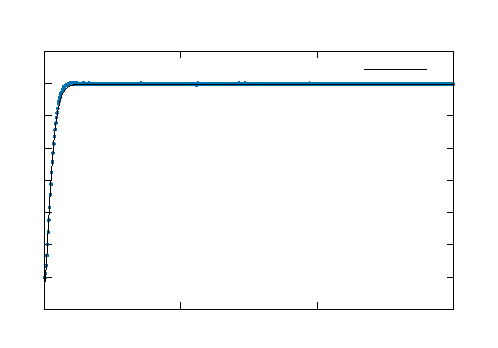
\includegraphics[width={223.20bp},height={151.20bp}]{kriticke}}%
    \gplfronttext
  \end{picture}%
\endgroup
 } \\
    \end{minipage} 
    \hfill
\end{table}
\vspace{-25pt}

\begin{table}[htpb]
    \hfill
    \begin{minipage}[b]{.4\linewidth}
        \centering
        \captionsetup{labelformat=empty}
        \caption{c) nadkritické tlumení}
        \vspace{-10pt}
        \resizebox{\textwidth}{!}{ \input{nadkriticke.tex} }
    \end{minipage} 
    \hfill
    \captionsetup{type=graph}
    \vspace{20pt}
    \caption{Měření přechodových jevů RLC obvodu pro různé odpory $ R_R $}
\end{table}


\begin{table}[htpb]
    \hfill
    \begin{minipage}[b]{.25\linewidth}
        \centering
        \begin{tabular}{l}
            \hline \hline
            3a\\
            \hline
            $f_0 = 1012.2 \pm 0.1$ Hz\\
            $\omega_0 = 6365.9 \pm 0.7$ Rad/s\\
            $\omega_d=6353.2 \pm 0.7$ Rad/s\\
            $\alpha=401.5 \pm 0.7$\\
            $R_R=20.42\ \Omega$\\
            $R=90.7 \pm 0.2\ \Omega$\\
            $ R_L \approx 16\ \Omega $ \\
            $ R_C \approx 3\ \Omega $ \\
            $R_{\rm celk}+R_G \approx 89 \ \Omega $\\
            \hline \hline
        \end{tabular}
        \captionsetup{labelformat=empty}
        \caption{3a) podkritické tlumení}
    \end{minipage}%
    \hfill
    \begin{minipage}[b]{.25\linewidth}
        \centering
        \begin{tabular}{l}
            \hline \hline
            3b\\
            \hline
            $ \alpha = 7050 \pm 20$ \\
            $R_R=1500$\\
            $R=1593 \pm 5$\\
            $ R_L \approx 11\ \Omega $ \\
            $ R_C \approx 10\ \Omega $ \\
            $R_{\rm celk}+R_G \approx 1571\ \Omega$\\
            \hline \hline
        \end{tabular}
        \captionsetup{labelformat=empty}
        \caption{3b) kritické tlumení.}
    \end{minipage}
    \hfill
    \begin{minipage}[b]{.25\linewidth}
        \centering
        \begin{tabular}{l}
            \hline \hline
            3c\\
            \hline
            $\alpha = 22490 \pm 20\ \Omega$\\
            $R_R=5000\ \Omega$\\
            $R=5082 \pm 5\ \Omega$\\
            $ R_L \approx 11\ \Omega $ \\
            $ R_C \approx 10\ \Omega $ \\
            $R_{\rm celk}+R_G=5071\ \Omega$\\
            \hline \hline
        \end{tabular}
        \captionsetup{labelformat=empty}
        \caption{3c) nadkritické tlumení.}
    \end{minipage}
    \hfill
    \caption{Výsledky zpracování přechodovýh jevů. $ R_G \approx 50 $  }
\end{table}

\section{Závěr}

Změřil jsem impedance a fázový posun jednoho odporu, cívky a kondenzátoru prvně pomocí RLC metru a potom jen pomocí osciloskopu. Výsledné hodnoty obou metod si přibližně odpovídají a lze je nalézt v tabulkách 1 a 2.

V druhé části jsem měřil impedanci a fázový posun nuceného kmitání sériového RLC obvodu v závislosti na fázové frekvenci budícího napětí. Hodnoty jsou vyneseny do grafů 1 a) a b), odkud jsem z fitu zpětně dopočítal impedance použitých součástek. Výsledky jsou v tabulce 2 a velmi dobře odpovídají měření z první části.

Nakonec jsem pro tuto cívku a kondenzátor měřil kritické, podkritické a nadkritické kmity, použitím odpovídajícího odporu $ R_R $ v sériovém obvodu. Změřené hodnoty jsou vynesené do grafů 2 odkud jsem fitoval tlumící faktor $ \alpha $, ze kterého lze zpátky dopočítat odpor obvodu. Získané hodnoty veličin jsou uvedeny v tabulce 9 a v rámci chyby sedí.


\end{document}
